\subsection*{Case 6} % SoftwareAG 
\label{case: 6}
% Inference architecture
\DIFaddbegin \begin{figure*}[b]
\centering
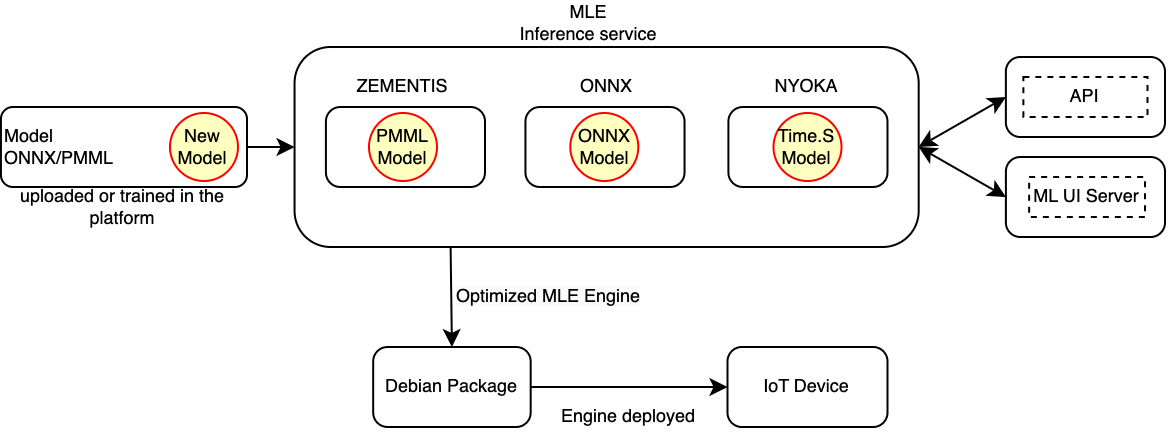
\includegraphics[width=\linewidth]{images/case6_deployment_process.png}
\caption{\DIFaddFL{Case 6 deployment setup}}
\label{fig: case6_deployment_process}
\end{figure*}

%DIF >  Inference architecture
\DIFaddend % \begin{figure*}[t]
% \centering
%DIF <  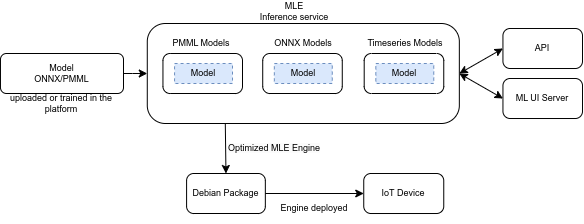
\includegraphics[width=0.8\textwidth]{images/case6_deployment_process_v2.png}
%DIF <  \caption{Case 6 deployment setup}
%DIF <  \label{fig: case6_deployment_process}
%DIF >  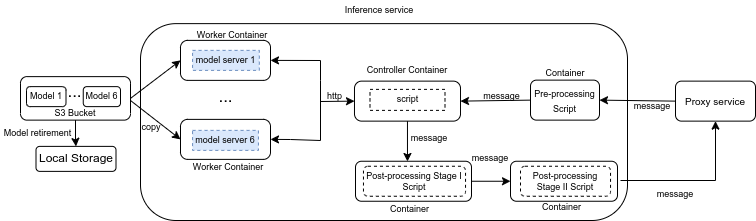
\includegraphics[width=0.9\textwidth]{images/case5_deployment_process_v2.png}
%DIF >  \caption{Case 5 Inference Architecture}
%DIF >  \label{fig: case5_deployment_process}
% \end{figure*}
\DIFdelbegin %DIFDELCMD < 

%DIFDELCMD < %%%
%DIF <  Inference architecture
%DIFDELCMD < \begin{figure*}[t]
%DIFDELCMD < \centering
%DIFDELCMD < 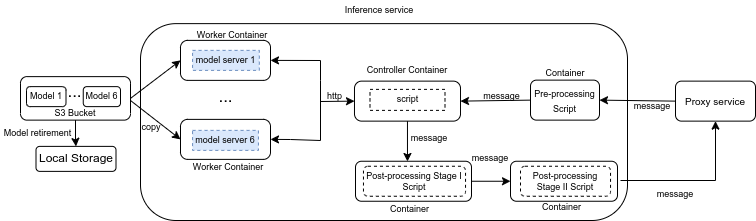
\includegraphics[width=0.9\textwidth]{images/case5_deployment_process_v2.png}
%DIFDELCMD < %%%
%DIFDELCMD < \caption{%
{%DIFAUXCMD
\DIFdelFL{Case 5 Inference Architecture}}
%DIFAUXCMD
%DIFDELCMD < \label{fig: case5_deployment_process}
%DIFDELCMD < \end{figure*}
%DIFDELCMD < %%%
\DIFdelend 

This case company develops an IoT fleet management platform that provides control, monitoring, analytics, and ML functionality for retrofitted or inbuilt sensors. We focused on the ML component of the platform, which offers model management, model training, and model deployment functionality. These functionalities are embedded in two modules: the machine learning workbench (MLW) and the machine learning engine (MLE), respectively. The MLE system handles deployment-related tasks. The entire ML system is accessible through a web interface to support low-code use cases and an API for programmable use cases. Each sub-module can be used independently, allowing users to adopt only the desired functionality and alternative external tools for other aspects of their ML workflow. The use of native Python scripts and Jupyter Notebooks are also supported for more programming-oriented users, which allows the use of more advanced modelling approaches, such as using neural networks. The entire platform is accessible through a web interface or a REST API. %The ML system contains multiple inbuilt time-series analysis algorithms that provide an autoML capability.

\textit{Pre-Deployment}: Models can be added to the platform in two ways: they can either be trained on the platform or uploaded as pre-trained models. However, these models need to be packaged in either PMML (Predictive Model Markup Language) or ONNX (Open Neural Network Exchange) formats which facilitate ML framework and hardware-agnostic deployments. Models are stored on the platform with no elaborate versioning mechanism. Instead, version management is implemented at the project level, where various artefacts belong to a given project. Models can be in one of two states: active or inactive. An active model is kept in memory, while an inactive model is stored in a colder location and removed from memory. It is also possible to delete a model entirely if desired. If multiple model versions are needed, they can be stored as a model group, allowing the models to be managed together. 

\textit{Quality Assurance}: During the model import and conversion process, the platform has a parser that checks the uploaded model's file for semantic errors and makes automatic corrections. Some parsing errors still require manual resolution. The system’s workflow does not include quality assurance steps or integrations. Such would need to be handled outside of the system. %

\textit{Server Environment}: The MLE, the platform's inference engine, handles deployment-related functions. The system is composed of four main microservices: i) zementis, which serves and manages PMML-based models; ii) ONNX, which serves and manages ONNX-based models; iii) nyoka, which provides time-series and clustering models; iv) machine-learning, a web user interface that provides interaction points to the rest of the micro-services. These components are shown in Figure~\ref{fig: case6_deployment_process}. A programmatic interaction with the MLE system is also available as an API, allowing greater flexibility and facilitating integration with other systems.

Since MLE and the rest of the components are provided as a hosted platform, other low-level issues related to infrastructure provisioning, virtualization, runtime, and application containerization are eliminated from the developer’s workflow.

For IoT deployment, the platform generates an optimized version of the MLE runtime as a Debian package. This package is installed on the target IoT devices and the model artefacts for inference.

\textit{Inference}: The platform supports online and batch inference through REST APIs. In batch inference scenarios, the input size is limited to 500MB, and results are returned as a compressed zip file. 

ONNX models support more complex inference workflows by having inference pipeline objects which consist of pre/post-processing steps and inference. The pre/post-processing steps are implemented as scripts, and the inference results are packaged into JSON format. For example, such a process is used in an edge computer vision task.

By default, a model trained in the platform is deployed to the MLE engine, considered a cloud deployment. Inference can be carried out through an API call or the web interface. Models deployed to IoT or edge devices provide inference using the runtime’s command line tool directly on the device.

%The platform provides an API to generate a time series model for inference. This process is implemented as an asynchronous call that returns a status URL which the calling entity can periodically query for the model's status. The model can provide inference from the cloud (MLE) engine or be downloaded and installed on an edge device.

\textit{Monitoring}: The platform provides an API to access a model’s memory footprint and prediction scoring metrics. The scoring metrics are cumulative of the various versions of the model and only available for classification and regression models.